\documentclass{beamer}
\usepackage{mathrsfs}  
\usepackage{xcolor}
\usepackage{setspace}
\usepackage{comment}
\usepackage[utf8]{inputenc}
\usepackage[T1]{fontenc}

% config du thgeme metropolis
\usetheme[progressbar=frametitle,block=fill, titleformat=smallcaps,sectionpage=progressbar,]{metropolis}



\title{Module d'Analyse Statistique : Introduction générale}
\subtitle{M2 IGAST}
\date{2021-2022}
\author{Paul Chapron \textsuperscript{1} }
\institute{ \textsuperscript{1}LASTIG-UGE-IGN/ENSG}



%definition de la couleur du texte dans la balise \alert{}
\definecolor{vertIGN}{HTML}{96C31E} % vert IGN %vrai valeur #97BE0D
\setbeamercolor{alerted text}{fg=vertIGN}

\definecolor{grisIGN}{HTML}{22292F} % Gris IGN tiré vers le noir 
\setbeamercolor{background canvas}{bg=grisIGN}




% code pour placer le log ENSG dans le bandeau de titre 
\makeatletter
\setbeamertemplate{frametitle}{%
  \nointerlineskip%
  \begin{beamercolorbox}[%
      wd=\paperwidth,%
      sep=0pt,%
      leftskip=\metropolis@frametitle@padding,%
      rightskip=\metropolis@frametitle@padding,%
    ]{frametitle}%
  \metropolis@frametitlestrut@start%
  \insertframetitle%
  \nolinebreak%
  \metropolis@frametitlestrut@end%
  \hfill
  \raisebox{-0.6ex}{
\includegraphics[height=4ex,keepaspectratio]{img/logoENSG_small.jpg}}
  \end{beamercolorbox}%
}
\makeatother




% logo ENSG première page 
\titlegraphic{\vspace{4cm}\flushright
\includegraphics[width=2cm,height=2cm]{img/logoENSG_big.png}} 



\begin{document}
\metroset{background=dark} % change background theme according to manual
\maketitle	

\section{Introduction Générale} 

\begin{frame}{Références}

\begin{itemize}
\item Cours M2 IGAST 2018 d'Ana-Maria Olteanu-Raimond 
\item R et espace \url{https://framabook.org/r-et-espace/}
\item Probabilités, analyse de données et statistiques , Gilbert Saporta, Editions TECHNIP, 2011
\item Cours de H. Commenges \url{https://gitlab.huma-num.fr/hcommenges/cours_statcomplet/-/raw/master/cours_statcomplet.pdf}
\item Nombreuses ressources en ligne, e.g. : 
\item \url{http://www.foad-mooc.auf.org/IMG/pdf/424B_-Application_des_methodes_statistiques_d_analyse.pdf}
\item \url{http://www.itse.be/statistique2010/co/Module_statistique_FSP.html}
\end{itemize}
 

\end{frame}







\begin{frame}{Analyse spatiale : définition} 


L’analyse spatiale étudie la \alert{répartition} et l’\alert{organisation} d’ensembles d’objets qui sont \alert{localisés}  

L’objectif est de : 

\begin{quote}
«déceler en quoi la localisation apporte un élément utile à la connaissances des objets étudiés et peut en expliquer les caractéristiques» 

[Pumain, Saint-Julien 97] 
\end{quote}
\end{frame}


\begin{frame}{ Spécificité de l'analyse \textbf{spatiale}}

\begin{block}{Analyse statistique}

Méthodes \alert{résumant} et \alert{généralisant} des observations
\begin{itemize}	
\item Les unités d’analyse sont des éléments indépendants en principe 
\item On ne s’intéresse pas à leur localisation ni à leur intéractions (spatiales)
\end{itemize}
\end{block}
\vfill
\begin{block}{Analyse \alert{spatiale} statistique} 
\begin{itemize}
  \item Les unités d’analyse sont localisables 
  \item On s’intéresse à leur propriétés y compris la localisation
  \item On fait l’hypothèse que leur localisation peut influencer les valeurs observées
\end{itemize}
\end{block}

\end{frame}


\begin{frame}{Données spatiales vs. non spatiales }

Données spatiales :
  
  Individus restreints spatialement (\alert{selection spatiale}), ou variables de \alert{localisation} géographique (e.g. Lieu de résidence, coordonnées) renseignées pour les individus 
  
  
  
  quid des \alert{distances} ? $\rightarrow$ modèle gravitaire , réseau etc.

\end{frame}


\begin{frame}{Deux approches} 
\begin{block}{Analyse géométrique :} 

approche \alert{géométrique} pour mieux décrire les données: analyse de forme, de réseaux, de proximité, méthodes de création de nouvelles entités à partir de la géométrie des objets
\end{block}
\vfill
\begin{block}{Analyse de données  :} 

approche \alert{statistique} permettant de faire émerger des relations (des groupes, des lois)  pour aider  l’étude de certains phénomènes
\end{block}
\end{frame}


\section{Statistiques Inférentielles vs. Statistiques Descriptives}


\begin{frame}{ Statistiques Inférentielles}  




  A partir d'un échantillon , que peut-on attendre (=\alert{inférer}) de la population ?
\begin{itemize}
  \item Modèles, estimateurs, ... : \alert{régression}, \alert{estimation}, \alert{extrapolation}
  \item e.g. sondages, recensement 
\end{itemize}

\end{frame}  
  
\begin{frame}{Statistiques inférentielles : exemple}
  


\begin{figure}
  \centering
     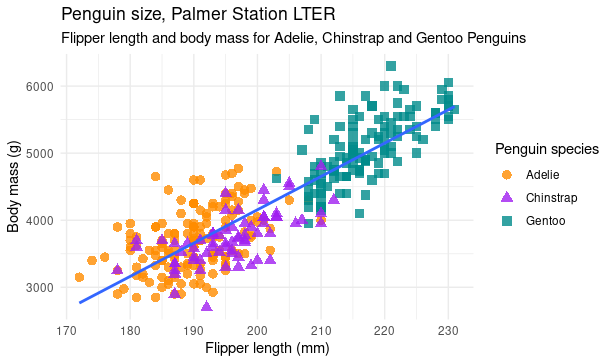
\includegraphics[width=.7\linewidth]{img/penguins_reglin.png}
\end{figure}

  
\begin{small}
\begin{spacing}{0.75}
Penguins data were collected and made available by Dr. Kristen Gorman and the Palmer Station, Antarctica LTER, a member of the Long Term Ecological Research Network.
[https://github.com/allisonhorst/palmerpenguins]
\end{spacing}
\end{small}
\end{frame}

\begin{frame}{Statistiques Descriptives} 
Décrire, résumer, synthétiser  les propriétés d'une \alert{population} à partir des \alert{variables} qui décrivent ses individus.

\begin{itemize}  
\item \alert{Graphiques} : nuages de points , histogramme, ...
\item \alert{Mesures} (fréquences, distributions, moments) sur des variables
\item \alert{Liaisons} statistiques entre variables : corrélation, covariance,...
\item \alert{Structure} interne des données : classification , ACP,...
\end{itemize}

\end{frame}

\begin{frame}{Dans ce module} 


Nous ferons majoritairement de la statistique \alert{descriptive}

(même si, pour bien décrire, il faut parfois inférer)

\end{frame}

\section{Vocabulaire }


 
\begin{frame}{Population}

 \alert{Ensemble} d'individus  
 
 "données", "corpus", "échantillon", "data"
 

très souvent \alert{tabulaires} 
\end{frame}
 
\begin{frame}{Individus}

 \alert{Unité} statistique \alert{élémentaire}: personnes, logements, ...
 
 
  $\rightarrow$ "les lignes du tableau"

\end{frame}

\begin{frame}{Variables} 


 \alert{Caractéristiques, propriétés} d’un individu, mesurées par des enquêtes, des observations...


$\rightarrow$ "les colonnes du tableau"  


\end{frame}


\begin{frame}{Types de variables}


\alert{Qualitatives} : facteurs e.g. couleur, genre, CSP, type de pokemon,... 
  $\rightarrow$ notion de \alert{modalité}
 
\alert{Quantitatives} : nombres e.g. taille, masse, revenu, surface, points de vie,...  
$\rightarrow$ parfois exprimées avec des \alert{unités} : m, kg, s



\end{frame}



\begin{frame}{Attention aux groupes !  (paradoxe de Simpsons)}



Paradoxe de Simpsons

\begin{small}
source: wikipedia
\end{small}

\end{frame}





\begin{frame}{Discrètes et Continues}

Variables quantitatives \alert{continues} : $var \in \mathbb{R}$

Valeurs réelles,  toutes les valeurs de l'intervalle de mesures peuvent exister 


Variables quantitatives \alert{discrètes} : $var \in \mathbb{N}$ 

Valeurs entières, pour des attributs \alert{dénombrables} (comptage) , 

parfois utilisées pour encoder une variable qualitative à deux modalités e.g. présence (1) , absence(0)

\end{frame}


\begin{frame}{Variables \alert{qualitatives} }

les valeurs sont prises dans un ensemble \alert{fini} de valeurs possibles, défini par \alert{extension} (i.e. on donne la liste des valeurs possibles)


$\rightarrow$ notion de \alert{modalités} 


$\rightarrow$ \alert{nominales} (non ordonnées e.g. état civil ) ou \alert{ordinales} (ordonnées e.g. échelle de Lickert) 


\end{frame}


\begin{frame}{l'Échelle d’Analyse}


Spécificité de la statistique spatiale : à quelle échelle observer ? 

Quel découpage, quelles unités spatiales ?

«Problème insoluble» : le \alert{MAUP} (Modifiable Areal Unit Problem)

\end{frame}

\begin{frame}{Unités spatiales }

\alert{Mailles administratives} : 

agrégation/imbrication d’unités spatiales prédéfinies : comtés, départements, régions, pays

e.g. Comprendre comment  le taux de chômage d’un pays est distribué entre les régions pour guider les politiques économiques


\alert{Découpages}: 

identification d'unités spatiales ayant des caractéristiques semblables

e.g. IRIS, carroyage 

\end{frame}


\begin{frame}{ Échelle individuelle vs. Échelle agrégée }

\alert{Désagrégation} ou  \alert{Ventilation} 


  $\rightarrow$ Inférer des caractéristiques individuelles à partir de l’analyse de données agrégées (ni facile ni immédiat)


\alert{Agrégation} 


$\rightarrow$ Inférer des caractéristiques concernant les unités agrégées d’après les caractéristiques individuelles 

\end{frame}

\begin{frame}{ le MAUP (Modifibale Aereal Unit Problem)}

Problème d'agrégation spatiale : les résultats d'une analyse statistique spatiale dépendent du choix d'agragation 

biais «sytématique et insoluble» 

Exemples tirés du rapport ESPON : \url{https://www.espon.eu/sites/default/files/attachments/espon343_maup_final_version2_nov_2006.pdf}

\end{frame}

\begin{frame}{MAUP exemple 1}


<div style="text-align:center">
<img src="./Maup1.png" width=100% >
</div>

\end{frame}
\begin{frame}{MAUP exemple 2}

<div style="text-align:center">
<img src="./Maup2.png" width=100%>
</div>

\end{frame}
\begin{frame}{La première" chose à faire "}

Représenter/Tracer/Cartographier  les variables de la population !

\end{frame}

\begin{frame}{}

Attention aux seules valeurs chiffrées : exemple du "dinosaure"

\end{frame}


\end{document}
